\documentclass[conf]{new-aiaa}
%\documentclass[journal]{new-aiaa} for journal papers
\usepackage[utf8]{inputenc}
\usepackage{graphicx}
\usepackage{amsmath}
\usepackage{subcaption}
\usepackage{sidecap}
\usepackage{listings}
\usepackage[version=4]{mhchem}
\usepackage{siunitx}
\usepackage{longtable,tabularx}
\setlength\LTleft{0pt} 



\title{A Convex Optimal and LQG Control Approach for Quadrotors}
\author{Pádraig Lysandrou
\footnote{Undergraduate Student, Electrical and Computer Engineering, AIAA Student Member \\ A final project for MAE6780: Multivariate Control Theory}}
\affil{Cornell University, Ithaca, New York, 14853}
\begin{document}
\maketitle
\pagenumbering{gobble}

\begin{abstract}
In this paper, I present the theory behind and implementation of a neighboring optimal Linear Quadratic Gaussian quadrotor controller with convex optimal guidance trajectories. My LQG solution uses an Extended Kalman Filter for optimal nonlinear estimation. I employ the convex optimization machinery as the guidance algorithm to generate paths of minimum energy consumption. This work is motivated by applications which require efficient use of energy. This includes autonomous delivery, mapping missions, search and rescue, swarm path planning, and many more. The ultimate goal of this project was to design and simulate a functioning LQG controller that follows convex optimal trajectories with high accuracy and amenable to implementation on my own physical autonomous hardware platforms. I would like my solution to be extensible to more complicated tasks in the future.
\end{abstract}


\section*{Nomenclature}

{\renewcommand\arraystretch{1.0}
\noindent\begin{longtable*}{@{}l @{\quad=\quad} l@{}}
$A$ & Linearized state space dynamics matrix\\
$B$ & Linearized state space input matrix\\
$C$ & Observation Matrix \\
$\Sigma_{t|t}$ & State covariance matrix at time $t$ with information known at $t$\\
$\mathbf{x}$ & State vector\\
$\mathbf{u}$ & Input vector\\
$\Sigma_w$ &Process noise covariance matrix\\
$\Sigma_v$ & Observation noise covariance matrix \\
$\mathbb{E}[]$ &Expected value operator \\
$\min$ &Minimization operator \\
$Q$ &State penalty matrix \\
$R$ &Input penalty matrix \\
\end{longtable*}}


\clearpage
\begin{doublespace}
\pagenumbering{arabic}

\section{Introduction and Theory}
The goal of this project was to design and simulate a functioning LQG controller that follows convex optimal trajectories with high accuracy. Additionally, I wanted the algorithm to be amenable to implementation on my own quadrotor platforms. To reach this goal, I chose a control solution that could be implemented online and would be simple to implement on an embedded system such as an ARM Cortex microcontroller with interrupt service routine timers. Due to Wonham's separation principle, which I will discuss later, the LQG controller can be split up into an optimal regulator (LQR) and an optimal estimator in the form of a Kalman Filter. If both are stable, then the whole control solution is stable. In my implementation, I write my own finite-time-horizon LQR using the Riccati matrix equation. Additionally, I have written my own Extended Kalman Filter (EKF) utilizing nonlinear state propagation via our dynamical equations. For the theory section, I will be covering the quadrotor dynamics, derivation of the LQG controller, introducing convex optimization, and the derivation of my own convex problem proposition.
\subsection{Dynamics of the Quadrotor}
Before we develop the control system, we must first create a dynamic model for the system. The frame of the vehicle is a cross-shape with four motor/propeller combinations, one on each end. In figure \ref{fig:f1}, we see that if we increase the thrust similarly on F1/F2 or F3/F4 the vehicle rolls right or left respectively, as a torque is applied to the system. Additionally we see that if we increase the thrust produced by F4/F1 or F3/F2 the quadrotor pitches forward or backward respectively. The rotor speeds can be increased or decreased to produce a yaw on the vehicle with the conservation of angular momentum. 

\begin{singlespace}
\begin{SCfigure}[1][!h]
	\begin{minipage}{0.5\textwidth}
	\centering
	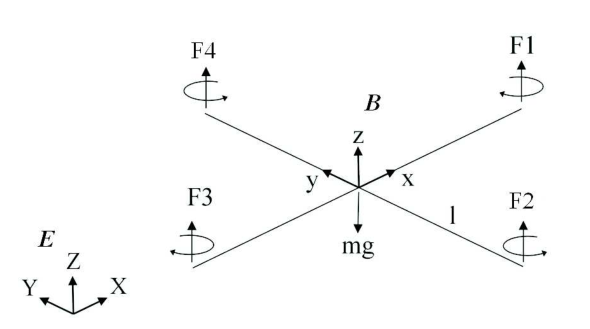
\includegraphics[scale= 0.45]{quad.png}
	\end{minipage}
	\begin{minipage}{0.5\textwidth}
		\begin{tabular}{| l | c |}
		  \hline			
		  $\xi$ & position vector\\
		  $R$ & direction cosine matrix\\
		  $\hat{\omega}$ &skew symmetric angular rate matrix\\
		  $\phi,\theta,\psi$ & roll, pitch, yaw\\
		  $x,y,z$ & inertial position\\
		  $\Omega_i$ & rotor speed\\
		  $I_x,y,z$ & body inertia\\
		  $J_r$ & rotor inertia\\
		  $b$ & thrust factor\\
		  $d$ & drag factor\\
		  $l$ & lever arm\\
		  $g$ & gravitational acceleration\\
		  \hline  
		\end{tabular}
	\end{minipage}
\end{SCfigure}
\begin{figure}[!h]
	\caption{Quadrotor Layout with body fixed frame B and inertial frame E and notation reference from \citep{ICRApaper}}
	\label{fig:f1}	
\end{figure}
\end{singlespace}


\begin{singlespace}
\begin{SCfigure}[1][!ht] 
	\begin{minipage}{0.25\textwidth}
		\begin{equation*}
			\begin{cases}
				& \dot{\xi} = \nu \\
				& m\dot{v} = RF_b \\
				& \dot{R} = R\hat{\omega} \\
				& J\dot{\omega} = -\omega \times J\omega + \tau_a
			\end{cases}
		\end{equation*}
	\end{minipage}
  \begin{minipage}{.4\textwidth}
    \begin{align*}
        &\ddot{x}=(\cos\phi\sin\theta\cos\psi + \sin\phi\sin\psi)\frac{U_1}{m} \\
		&\ddot{y}=(\cos\phi\sin\theta\sin\psi - \sin\phi\cos\psi)\frac{U_1}{m} \\
		&\ddot{z}=(\cos\phi\cos\theta)\frac{U_1}{m} -g \\
		&\ddot{\phi} = \dot{\theta}\dot{\psi}\Big(\frac{I_y - I_z}{I_x}\Big) - \frac{J_r}{I_x}\dot{\theta}\Omega + \frac{l}{I_x}U_2\\
		&\ddot{\theta} = \dot{\phi}\dot{\psi}\Big(\frac{I_z - I_x}{I_y}\Big) - \frac{J_r}{I_y}\dot{\phi}\Omega + \frac{l}{I_y}U_3 \\
		&\ddot{\psi} = \dot{\phi}\dot{\theta}\Big(\frac{I_z - I_y}{I_z}\Big) + \frac{1}{I_z}U_4
    \end{align*}
  \end{minipage}%
  \begin{minipage}{.35\textwidth}
  	\begin{align*}
  		&U_1 = b(\Omega_1^2+\Omega_2^2 + \Omega_3^2 +\Omega_4^2)\\
  		&U_2 = b(\Omega_4^2-\Omega_2^2) \\
  		&U_3 = b(\Omega_3^2-\Omega_1^2) \\ 
  		&U_4 = d(\Omega_2^2+ \Omega_4^2 - \Omega_1^2 - \Omega_3^2) \\ 
  		&\Omega = \Omega_2 + \Omega_4 - \Omega_1 - \Omega_3
  	\end{align*}
  \end{minipage}
\end{SCfigure}
\begin{figure}
	\caption{Governing Nonlinear Coupled Dynamical Equations}
    \label{eq1}
\end{figure}
\end{singlespace}

$U_1, U_2, U_3, U_4,$ and $\Omega$ represent the inputs of the system: total thrust, roll thrust, pitch thrust, and yaw thrust. The first set of equations in the curly braces (\textbf{equations \ref{eq1}}) show the overall simplified dynamics. Once the  thrust is distributed in the inertial frame, we can write the dynamics as the second set of equations shown. These are nonlinear, 6 degree of freedom, coupled dynamical equations. The set of equations on the far right describes these forces in rotor speeds $\Omega_i$. Keep in mind that $U_i$ is not the force from each motor, but follows these equations. Additionally, looking at the simplified second order derivative equations, we see that the translational accelerations are dependent on the attitude dynamics, but the attitude dynamics do not depend on the translational dynamics. Therefore, we can model our dynamics as two subsystems with one dependency. Rewriting in state space form as $\dot{\mathbf{x}}= f(\mathbf{x},\mathbf{U})$, with $\pmb{x}= (x_1 ... x_{12})^T$ as the state vector, we have \textbf{\ref{eq2}}. 
\begin{singlespace}
\begin{SCfigure}[1][!ht] 
	\begin{minipage}{0.3\textwidth}
		\begin{align*}
		\pmb{x}=
			\begin{cases}
				& x_1 = x \\
				& x_2 = \dot{x_1} = \dot{x} \\
				& x_3 = y \\
				& x_4 = \dot{x_3} = \dot{y}\\
				& x_5 = z \\
				& x_6 = \dot{x_5} = \dot{z}\\
				& x_7 = \phi \\
				& x_8 = \dot{x_6} = \dot{\phi}\\
				& x_9 = \theta \\
				& x_{10} = \dot{x}_9 = \dot{\theta}\\
				& x_{11} = \psi \\
				& x_{12} = \dot{x}_{11} = \dot{\psi}
			\end{cases}
		\end{align*}
	\end{minipage}
  \begin{minipage}{.4\textwidth}
  	\[
	\therefore f(\pmb{x},\pmb{U}) =
	\begin{bmatrix}
		& x_2 \\
        &(\cos x_7\sin x_9\cos x_11 + \sin x_7\sin x_11)\frac{U_1}{m} \\
        & x_4 \\
		&(\cos x_7\sin x_9\sin x_11 - \sin x_7\cos x_11)\frac{U_1}{m} \\
		& x_6 \\
		&(\cos x_7\cos x_9)\frac{U_1}{m} -g \\
		& x_8 \\
		&x_{12} x_{10}\Big(\frac{I_y - I_z}{I_x}\Big) - \frac{J_r}{I_x}x_{10}\Omega + \frac{l}{I_x}U_2\\
		& x_{10} \\
		&x_{12} x_8 \Big(\frac{I_z - I_x}{I_y}\Big) - \frac{J_r}{I_y}x_8 \Omega + \frac{l}{I_y}U_3 \\
		& x_{12} \\
		&x_{10} x_8\Big(\frac{I_z - I_y}{I_z}\Big)+ \frac{1}{I_z}U_4
	\end{bmatrix} \]
  \end{minipage}%
\end{SCfigure}
\begin{figure}[!h]
	\caption{State space form of dynamics}
    \label{eq2}
\end{figure}
\end{singlespace}

\subsection{LQG derivation}
We will derive the canonical linear quadratic Gaussian control problem using dynamic programming and backwards induction. First let us describe the system as the following linear time varying state space system. In a later part of this document, we will work with continuous time, linear time-invariant solution. For now we shall propose that $\forall t \in (0 ...T-1)$:


\begin{singlespace}
\begin{align}
& x_{t+1} = A_t x_t + B_t u_t + w_t \\
& y_t = C_t x_t + D_t u_t + v_t
\label{eq3}
\end{align}
\end{singlespace}


Where $\mathbb{E}[w_t]=\mathbb{E}[v_t]=0$. We attribute the cost-to-go structure of $c_t(x_t,u_t) = x_t^T Q_t x_t + u_t^T R_t u_t$ and a terminal cost structure of $c_T(x_T)= x_T^T Q_T x_T$ for $Q_t \geq 0$ positive semidefinite, $R_t > 0$ positive definite to imply convexity in cost. The positive definiteness of $R_t$ gives us required invertibility. Therefore, our cost function is as follows: 
\begin{singlespace}
\begin{equation}
{{\displaystyle J(\mathbf{x},\mathbf{u})=\mathbb {E} \left[{\mathbf {x} }_{N}^{\mathrm {T} }Q_T{\mathbf {x} }_{N}+\sum _{i=0}^{N-1}(\mathbf {x} _{i}^{\mathrm {T} }Q_{i}\mathbf {x} _{i}+\mathbf {u} _{i}^{\mathrm {T} }R_{i}\mathbf {u} _{i})\right]}}
\end{equation}
\end{singlespace}

As an aside, let's notice how we can encode reference tracking objectives, with $\hat{x}$ given as a trajectory, as $c_t(x,u)=||x_t - \hat{x}_t||_2^2$. We see that $||x_t - \hat{x}_t||_2^2 = x_t^Tx_t - 2\hat{x}_t^Tx_t + \hat{x}_t^T\hat{x_t}$ and can generate an augmented state vector as $\tilde{x}=[x_t 1]^T$. This is such that the following exists:
\begin{singlespace}
\begin{equation}
||x_t - \hat{x}_t||_2^2 =
\begin{bmatrix} x_t\\ 1 \end{bmatrix}^T
\begin{bmatrix} I_{nxn} &-\hat{x}_t \\ -\hat{x}_t^T &\hat{x}_t^T\hat{x}_t\end{bmatrix}
\begin{bmatrix} x_t \\ 1\end{bmatrix}
= \tilde{x}_t^T \tilde{Q}_t \tilde{x}_t
\end{equation}
\end{singlespace}

Let's leave this aside for now and see where the backwards inductive dynamic programming approach to solving this function takes us.
\subsubsection{Generating an Optimal Feedback Policy and Deriving the Riccati Equation via Dynamic Programming}
Let's star by evaluating the cost function backwards in time from the finite-time-horizon. The Hamilton-Jacobi-Bellman minimization functions, or optimal costs at each step, will be be referred to with the notation: $V_i^\star$. We will also show this for a linear time-varying system without loss of generality. I will also drop the timing subscripts for the state and input vectors for brevity, but they should be clear from the subscripts found in the function dependencies.
\begin{align}
&\textbf{Stage T:} \quad V_T^\star = \mathbf{x}^TQ_T\mathbf{x}  \\
&\textbf{Stage T-1:} \quad V_{T-1}^\star(\mathbf{x}_{T-1},\mathbf{u}_{T-1}) = \min_{\mathbf{u} \in \mathbb{R}^m} \mathbb {E} \left[\mathbf{x}^TQ_{T-1}\mathbf{x} + \mathbf{u}^TR_{T-1}\mathbf{u} + V_T^\star(A_{T-1}\mathbf{x} + B_{T-1}\mathbf{u} + \mathbf{w}_{T-1}) \right] \\
& = \mathbf{x}^TQ_{T-1}\mathbf{x} + \min_{\mathbf{u} \in \mathbb{R}^m} \mathbb{E} \left[\mathbf{u}^TR_{T-1}\mathbf{u} + (A_{T-1}\mathbf{x} + B_{T-1}\mathbf{u} + \mathbf{w}_{T-1})^TQ_T(A_{T-1}\mathbf{x}+ B_{T-1}\mathbf{u} + \mathbf{w}_{T-1})  \right] \\
& = \mathbf{x}^T(Q_{T-1} + A_{T-1}^TQ_TA_{T-1})\mathbf{x} + \mathbb{E}\left[w_{T-1}^TQ_Tw_{T-1} \right] + \min_{\mathbf{u} \in \mathbb{R}^m} \left[ \mathbf{u}^T(B_{T-1}^TQ_TB_{T-1} + R_{T-1})\mathbf{u} + \mathbf{x}^TA^TQ_TB\mathbf{u} \right]
\label{eqn4}
\end{align}

Here we were able to split apart the equation in deterministic and stochastic quantities. Additionally, we can see that the matrix equation between the $\mathbf{x}^T...\mathbf{x}$ terms is positive semi-definite, and therefore the whole term is convex. The term inside the minimization of equation \ref{eqn4} will be called $f(u)$ going forward. The first term of $f(u)$, between  $\mathbf{u}^T...\mathbf{u}$ is positive definite and the second term is affine in $u$. Therefore, the minimization is quadratic in $u$ and strictly convex due to positive definiteness. Let's minimize by using the gradient:
\begin{singlespace}
\begin{align}
&\nabla_u f(u) = 2(B_{T-1}^TQ_TB_{T-1} + R_{T-1})\mathbf{u} + 2B_{T-1}^TQ_TA_{T-1}\mathbf{x} = \mathbf{0} \\
&\therefore \mathbf{u}^\star = -(B_{T-1}^TQ_TB_{T-1} + R_{T-1})^{-1}(B_{T-1}^TQ_TA_{T-1})\mathbf{x}
\end{align}
\end{singlespace}

Where we have clearly found an optimal, Markovian, feedback policy of the form $\mathbf{u}_{T-1}^\star = L_{T-1}\mathbf{x}_{T-1}$. We can now simplify our cost structure, which will ease our notation for further stages, to the following:
\begin{singlespace}
\begin{align}
& V_{T-1}^\star(\mathbf{x}_{T-1}) = \mathbf{x}^TK_{T-1}\mathbf{x} + \mathbb{E}\left[w_{T-1}^TQ_Tw_{T-1}\right]\\
& \textbf{where} \quad K_{T-1} = A_{T-1}^T (Q_T - Q_TB_{T-1}(B_{T-1}^TQ_TB_{T-1} + R_{T-1})^{-1}B_{T-1}^TQ_T)A_{T-1}
\end{align}
\end{singlespace}

and continuing onward for one more stage
\begin{singlespace}
\begin{align*}
&\textbf{Stage T-2:} \quad V_T^\star(\mathbf{x}_{T-2},\mathbf{u}_{T-2}) =  \min_{\mathbf{u} \in \mathbb{R}^m} \mathbb{E} \left[\mathbf{x}^TQ_{T-2}\mathbf{x} + \mathbf{u}^TR_{T-2}\mathbf{u} + \Xi^TK_{T-1}\Xi \right] + \mathbb{E} \left[ w_{T-1}^TQ_Tw_{T-1} \right]\\
& \text{where the state propagation/prediction is} \quad \Xi = (A_{T-2}\mathbf{x} + B_{T-2}\mathbf{u} + w_{T-2})
\end{align*}
\end{singlespace}

This is unsurprisingly quadratic in $\mathbf{u}$ and again we can obtain from this the optimal policy $\mathbf{u}_{T-2}^\star = L_{T-2}\mathbf{x}_{T-2}$ where $L_{T-2} = -(B_{T-2}^TK_{T-1}B_{T-2} + R_{T-2})^{-1}(B_{T-2}^TK_{T-1}A_{T-2})$. You can continue this backward and inductively prove $L_t, \forall t \in [0 ... T]$. You will get the following
\begin{singlespace}
\begin{align}
& L_{t} = -(B_{t}^TK_{t+1}B_{t} + R_{t})^{-1}(B_{t}^TK_{t+1}A_{t}) \\
& K_T = Q_T\\
& K_t = A_{t}^T (K_{t+1} - K_{t+1}B_{t}(B_{t}^TK_{t+1}B_{t} + R_{t})^{-1}B_{t}^TK_{t+1})A_{t}  \quad \quad \quad \forall t \in [0 ... T-1] \label{eqn5}
\end{align}
\end{singlespace}

You will notice that \ref{eqn5} is the backwards recursive, finite-time-horizon, Riccati Matrix equation. It should be known that now the feedback policy $\mathbf{L}_t$ $\forall t$ can be computed offline and applied to the system. Additionally, for a linear time-invariant system, like ours: $A_t = A$, $B_t = B$, $Q_t = Q$, $R_t = R$ $\forall t$. There are two proofs I will leave out for brevity. The first is that as $T$ approaches infinity, $K$ stays positive semi-definite. The second is the stability margins on the LQG controller. I feel the latter is best summed up by the abstract of John C. Doyle's famous 1978 paper "Guaranteed Margins for LQG regulators" which reads "Abstract -- There are none."

\subsubsection{Derivation of the Optimal Estimator, Kalman Filter}
The second half of the LQG problem is optimal estimation. Our feedback control policy up to now had deterministic state feedback. However, the imperfectly observed system has the feedback policy $u_t^\star = L_t\mathbb{E}[x_t|I_t]$ where $I_t$ is all the sensor information gathered up until that point. Notice that the LQR gain is independent of the noise distribution. Similarly, we will find that the optimal estimate is independent of the control policy. This can be proved by Wonham's separation theorem which state that separately stable controller and estimator pairs are stable in closed loop. Our objective is to find $x_{t|t}=\mathbb{E}[x_t|I_t]$ given that the state and observation have independent, identically distributed Gaussian additive noise. Throughout the calculation we will keep track of both the state and $\Sigma_{t|t}$ the state covariance matrix. In the first step, we will predict the next state and state covariance matrix ($\mathbf{x}_{t+1|t}$ and $\Sigma_{t+1|t}$) given the current information and the known dynamics of the system. The second step involves filtering this and weighing between the sensor measurements and our own dynamic propagation. Once we generate the estimated state, we can do the algorithm again recursively.

\begin{singlespace}
\begin{align}
& \textbf{The Prediction Step}\\
&x_{t+1|t} = Ax_{t|t} + Bu_t \quad \text{in our case} \quad x_{t+1|t} = f(\mathbf{x}_{t|t},\mathbf{u}) \\ 
&\Sigma_{t+1|t} = A\Sigma_{t|t}A^T + G\Sigma_w G^T \\
& \textbf{The Filter Step}\\
&x_{t+1|t+1} = x_{t+1|t} + \Gamma_t (y_{t+1 - C_{t+1}x_{t+1|t}}) \\
&\Sigma_{t+1|t+1} = \Sigma_{t+1|t} - \Gamma_t C_{t+1}\Sigma_{t+1|t} \\ 
& \text{with Kalman Gain:}\quad \Gamma_t= \Sigma_{t+1|t}C_{t+1}^T(C_{t+1}\Sigma_{t+1|t} C_{t+1}^T + H_{t+1}\Sigma_vH_{t+1}^T)
\label{kalman} 
\end{align}
\end{singlespace}

However, in the implemented system, I have chosen to use the "Extended" Kalman filter. This is to say that instead of linearly propagating my dynamics, I use the full nonlinear equations ($\therefore x_{t+1|t} = f(\mathbf{x}_{t|t},\mathbf{u})$). However, I still have to linearize the system about a hovering point to be able to use the $A$ matrix in the covariance matrix propagation step.

\subsection{The Simple introduction to Convex Optimization}
The general form of an optimization problem is to find some $\displaystyle x^\ast \in \mathcal{X}$ such that $\displaystyle f(x^{\ast })=\min\{f(x):x\in {\mathcal {X}}\}$ in a feasible set $\mathcal{X}$.(\citep{boyd}) Posing the problem is usually the hard part, and rigorously proving that is convex such that it works with existing computational tools. Many times, the problem is non-convex and tricks like introducing slack variables and other forms of lossless convexification must be employed. Convex optimization problems usually look like:

\begin{singlespace}
\begin{align*}
& \textbf{minimize} &f(x) \\ 
& \textbf{subject to} &g_i(x) \leq 0, \forall i \\
& & h_{i}(x)=0, \forall i
\end{align*}
\end{singlespace}

for convex constraints in $g_i$ and affine equality constraints in $h_i$. I will talk about the problem that I have proposed and the software I used to solve it in the next section.








\section{Procedure - Step by Step}
\subsection{The Simulation and Dynamics Block}
To simulate the dynamics and design my controller, I used Simulink. The figure \ref{block} shows the full system and all of the constituent blocks. The center block labeled 'quadmodel' encases all of the system dynamics. I will focus on this for now.

\begin{figure}[!h]
\centering
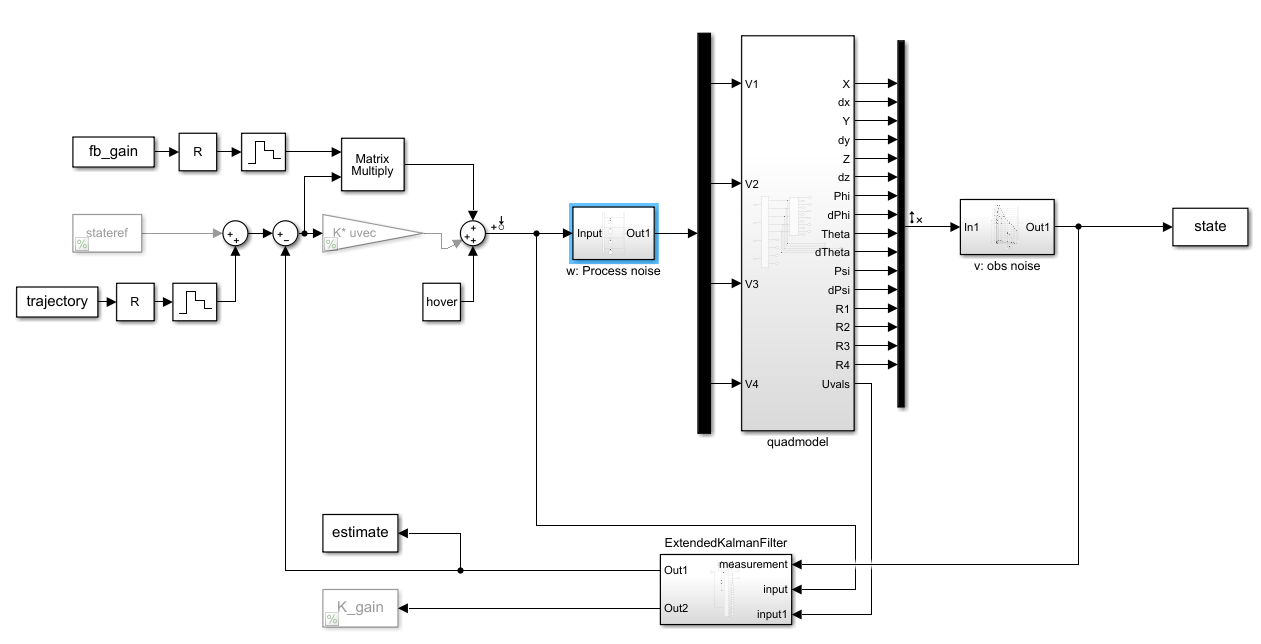
\includegraphics[scale= 0.45]{block.png}
\caption{Top Level Simulink block depicting all subsystems}
\label{block}
\end{figure}

Figure \ref{blocks} shows the full system dynamics blocks. Notice how the rotational dynamics are computed first which in turn motivate the translational dynamics. You will  notice that I also pipe out the rotor states and include them in my state vector. This is necessary for the linearization which I will cover in the next subsection. So now, my state vector is $\mathbf{x} \in \mathbb{R}^{16x1}$. The motor dynamics are linear and work out quite nicely when doing LQR.


\begin{figure}[!h]
\centering
\begin{subfigure}{.33\textwidth}
  \centering
  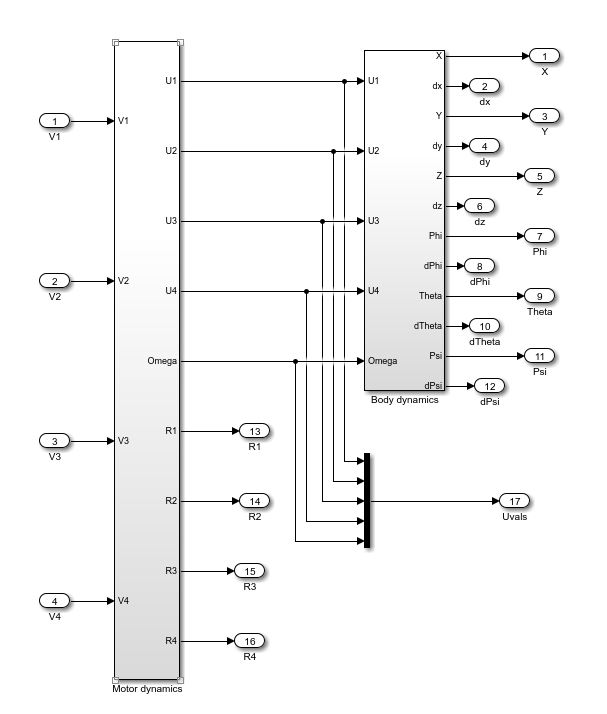
\includegraphics[scale= 0.3]{dynam.png}
  \caption{Higher level Block with motor and quad dynamics}
  \label{dynam}
\end{subfigure}%
\begin{subfigure}{.33\textwidth}
  \centering
  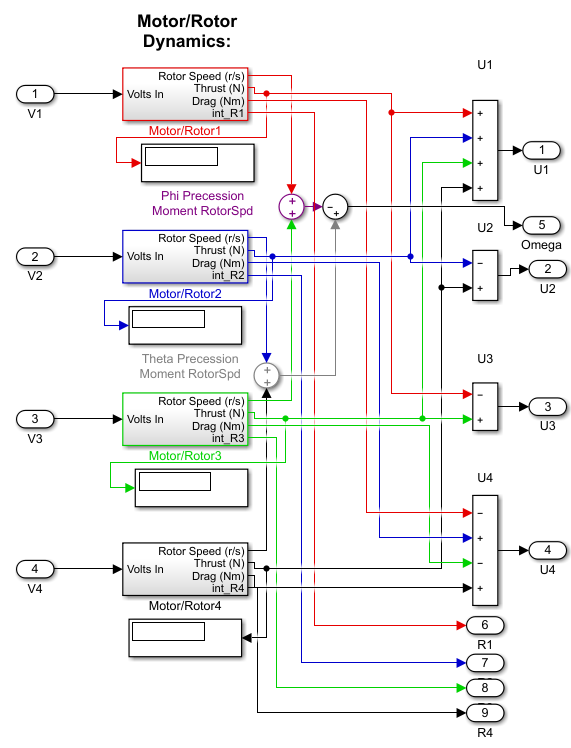
\includegraphics[scale= 0.35]{motdyn.png}
  \caption{Just the motor dynamics}
  \label{motdyn}
\end{subfigure}
\begin{subfigure}{.33\textwidth}
  \centering
  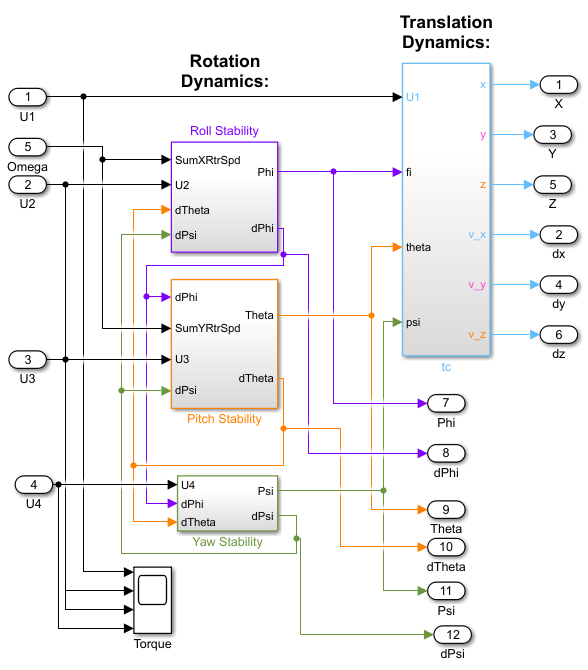
\includegraphics[scale= 0.35]{sysdyn.png}
  \caption{Just the quad dynamics}
  \label{sysdyn}
\end{subfigure}
\caption{All the subsystems within quadmodel}
\label{blocks}
\end{figure}



\subsection{LQR}
\subsubsection{Linearizing}
In order to use LQR, we must linearize the system about an equilibrium point. I did this about a stable hovering condition. I could have done this by hand by taking the derivative of each state with respect to each other as well as the inputs about that condition. This is very simple but would have been very tedious (at least $16^2$ derivatives). Therefore, once I build the model in MATLAB,  I used the linear systems tool box. I made an arbitrary loop, selected the input of the plant to be a perturbation input and the output to be an open loop output. I then went into the Linear Analysis application under $Analysis/Control Design$ and made sure my initial conditions, set by the integrators in the dynamics, were my hovering conditions. I then plotted the Bode diagrams which prompted the linear analysis to start. I saved the linear system model, which generated the standard (A,B,C,D) state space matrices, to my workspace and continued to used them for control design.

\subsubsection{The Regulator}
In order to come up with a trajectory following LQR solution, I used the finite time Riccati equation. I covered this earlier but showed the equation in discrete time. I certainly could have implemented it in this way but I chose to use the Riccati differential equation, which is the continuous time analog. We are very familiar with this and it takes the form:$-{\dot {P}}(t) = A^{T}P(t)+P(t)A-(P(t)B+N)R^{-1}(B^{T}P(t)+N^{T})+Q$ where the terminal cost matrix is the final value of the Riccati matrix P. I computed the gains offline and used them in my Simulink model. The gain matrices are invariant under the trajectory, and therefore the tuning process was one of making certain the controller could track small changes in error at each step continuing to the final time. 

\begin{singlespace}
\begin{lstlisting}[language=Matlab, caption = LQR Solve]
finalS = reshape(P,[16^2,1]);
[t,S] = ode45(@(t,S) rhs(t,S,A,B,R,Q), tspan, finalS);
for i = 1:length(tspan)
	Sii = reshape(S(i,:),16,16);
	Si(16*(i-1)+1 : 16*i,:) = Sii;
	j = length(tspan)-i+1;
	C((j*4)-3:j*4,:) = R\(B'*Sii);
	igain(j,:) = reshape(R\(B'*Sii),[1,4*16]);
end 
fb_gain = [flipud(tspan') igain];
\end{lstlisting}
\end{singlespace}

In listing 1 we see a small portion of the algorithm. I used the built-in Runge Kutte ODE solver to solve the differential Riccati equation. The RHS function is another function I wrote which lays out the equations and their derivative. Coming up with the P, Q, and R matrices was an iterative process which involved continuous simulation. I would increase the diagonal values of Q until the state was maintained well enough, with P arbitrarily high. I would then modify R to see how the control usage changed and if it better fit the type of tasks at hand, namely trajectory following. 

Keep in mind that this generate time-varying gain matrices. These must be reshaped and appended to a time-span vector to be used in Simulink. I make all of these edits in the initialization code that I run for the controller. This fact is also true for input trajectories.

\subsection{EKF}
In figure \ref{EKF} we see the Extended Kalman Filter block of my simulation. Instead of implementing this algorithm using discrete blocks, I found it easier to que a MATLAB function that I wrote. The algorithm I wrote in that block of code is identical to the recursive algorithm I have already discussed in \ref{kalman}. Notice that I use unit delays to feedback the state and covariance matrices back into the algorithm for the next time step. The unit delay block in Simulink is incredibly useful and allows you to even set initial conditions without fuss.

\begin{figure}[!h]
\centering
\begin{subfigure}{.33\textwidth}
  \centering
  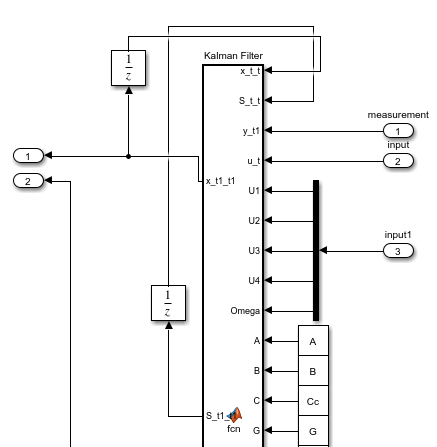
\includegraphics[scale= 0.4]{EKF.png}
  \caption{EKF Block which links to my MATLAB function}
  \label{EKF}
\end{subfigure}%
\begin{subfigure}{.33\textwidth}
  \centering
  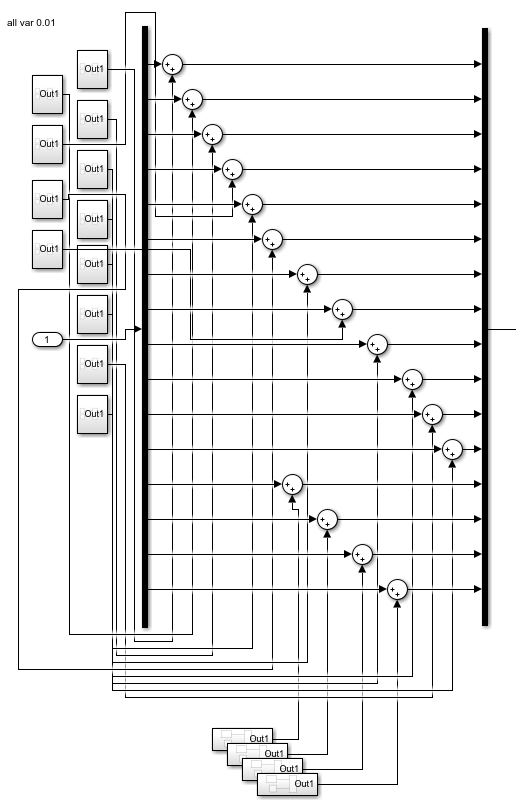
\includegraphics[scale= 0.35]{obsnoise.png}
  \caption{Observation additive noise block}
  \label{obsnoise}
\end{subfigure}
\begin{subfigure}{.33\textwidth}
  \centering
  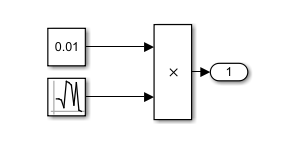
\includegraphics[scale= 0.5]{noise.png}
  \caption{Individual noise source}
  \label{noise}
\end{subfigure}
\caption{All parts of the optimal estimation block}
\label{ekfshit}
\end{figure}

In \ref{obsnoise} we see the independently, identically distributed, and additive noise segments that I put in the full state feedback path. I assume identical distribution on the original 12 states as if the sensor noise was relatively similar. I gave the rotor noise a much lower variance and amplitude. You can see in  \ref{block} that I did a similar thing for the process noise. In \ref{noise} we see how I implemented each of the source. I used a normal random variable. I changed the internal variance condition and multiplied it by a small constant to keep the amplitude within a reasonable range.

Tuning the EKF was particularly hard and took a lot of tinkering before it converged and worked with decent results. I made the $G$ and $H$ matrices identity for simplicity. I also set the diagonals of $\Sigma_v$ to the observation variances squared. Although I added process noise to the input stream, $\Sigma_w \in \mathbb{R}^{16x16}$, so I set it equal to $\Sigma_v$ for now. This seems to work quite well. I initially started the covariance matrix initial condition $\Sigma_{0|0}$ to be very high such that it converged downward. This was a mistake and did not converge as quickly as  I had expected. I now use the value: $\Sigma_{0|0} = 0.001*\mathbb{I}_{16}$ which seems to work very well. I will show all of these properties in the results section.


\subsection{The Convex Problem}
Proposing a convex control problem can be difficult. In most literature, convexity is shown rigorously using optimality conditions. In my situation, I simplify the problem to get rid of nonconvexities that arise in actuator dynamics. This means that I have modeled the four rotors as a single rotor that provides upwards thrust on the system that can be gimbaled. However, I keep actuator dynamic range constraints. Additionally, this thrust does not provide perturbations to the yaw. This is because trigonometric functions cannot be used in the objective or constraint functions as they are not convex. This made me simplify the dynamics even further to purely translational, and have the rotational states be unconstrained. You will also see that the dynamics is discretized. Moving forward, I will be using the CVX package in MATLAB to generate my trajectories.

The goal of the optimization problem is to use the least amount of control input from point to point. I can use equality constraints to set finite-time horizon setpoints and let the optimization machinery take care of everything in between. I shall use \citep{enhancements2008} as a literature example for this path planning algorithm. I will be simplifying it with quadrotor dynamics. Additionally, to make things easier, this will be a 'fuel-mass' minimization program that I am familiar with. So we pose the initial problem with a modified second problem:

\begin{singlespace}
\begin{SCfigure}[1][!h]
\begin{minipage}{0.5\textwidth}
	\begin{align*}
	& \textbf{Problem 1:} \\
	& \max_{t_f, T} m(t_f) = \min_{t_f, T}\int^{t_f}_0 \| \mathbf{u}(t)\| dt \\
	& \textbf{Subject to:} \\
	& \ddot{r}(t)= g + \frac{\boldsymbol u (t)}{m}, \quad \dot{m}(t)=-\alpha \| \mathbf{u}_c (t)\| \\
	& 0 \leq \lVert \mathbf{u} (t) \rVert \leq \rho_2 \\
	& m(0) = m_i, r(0) = r_0, \dot{r}(0) = \dot{r_0}, r(t_f) =\dot{r}(t_f) = 0
	\end{align*}
\end{minipage}
\begin{minipage}{0.5\textwidth}
	\begin{align*}
	& \textbf{Problem 2:} \\
	& \min_{t_f, T, \Gamma} \int^{t_f}_0 \| \Gamma(t) \| dt \\
	& \textbf{Subject to:} \\
	& \ddot{r}(t)= g + \frac{\mathbf{u} (t)}{m(t)}, \quad \dot{m}(t)=-\alpha \| \Gamma (t) \| \\
	& \| \mathbf{u}(t) \| \leq \Gamma(t) \\ 
	& 0 \leq \Gamma(t) \leq  \rho_2, \quad  r_z(t) > 0 \\
	& m(0) = m_i, r(0) = r_0, \dot{r}(0) = \dot{r_0}, r(t_f) =\dot{r}(t_f) = 0
	\end{align*}
\end{minipage}
\end{SCfigure}
\end{singlespace}

Where $r$ represents the position vector in a surface-fixed frame, $\mathbf{u}$ represents the total propeller force vector, and $\alpha$ represents the rate of change of fuel mass. Problem 2 is derived by introducing $\Gamma$ as a slack variable to the initial problem. $\Gamma$ replaces $\|\mathbf{u}\|$ with an additional constraint $\|\mathbf{u}(t)\| \leq \Gamma(t)$. Because this problem is a relaxation of the initial problem, Problem 1 defines a feasible solution of Problem 2. However, a feasible solution for problem 2 does not necessarily define one for Problem 1. Lemma 1 of \citep{ploen2007} shows that the optimal solution to Problem 2 also is a feasible solution of Problem 1. This is done by using the Hamiltonian of Problem 2 and using the necessary conditions for optimality, pointwise maximum principle, and the transversality condition. This paper shows, with lemma 1, that modified constraints of Problem 2, namely the scalar slack variable $\Gamma$ convexifies Problem 1. The lemma states that if there is an optimal solution to Problem 2, then there also exists one for Problem 1, and it can be found from the optimal solution of Problem 2. We also see that that the admissible set of controls for the second problem are within the set of admissible controls for the first. Together this means that Problem 2 can be solved with convex control constraints in order to find a solution to the nonconvex Problem 1. 


Now change of variables will allow for a much cleaner equation for expanding Problem 2 into the third form which will be a continuous time cone problem. Let us perform $\sigma = \frac{\Gamma}{m}$ and $u = \frac{\mathbf{u}}{m}$. Consequently the dynamics change to $\ddot{r}(t) = u(t) + g$, $\frac{\dot{m}(t)}{m(t)} = -\alpha\sigma(t)$
and clearly $m(t)= m_i\exp\big[-\alpha \int^{t_f}_0 \sigma(t)d\tau \big]$.

Therefore we must minimize the integral term in the last mass dynamical equations. The original constraints the follow that
\begin{singlespace}
\begin{align*}
& \|u(t)\| \leq \sigma(t), \quad \forall t \in [0,t_f] \\
& 0 \leq \sigma(t) \leq \frac{\rho_2}{m(t)}, \quad \forall t \in [0,t_f 
\end{align*}
\end{singlespace}


This inequality now describes a convex set. However, when we consider $m$ by itself to be variable of the problem, these inequalities become bilinear and do not define a convex region. We will now introduce $z$ to resolve this issue and convexify these inequalities. Lets define $z = \log{m}$. And then the fuel depletion rate now becomes $\dot{z}(t) = -\alpha\sigma(t)$.
The inequalities now become $ 0\leq \sigma(t) \leq \rho_2\exp{(-z(t))}. \quad \forall t \in [0, t_f]$

The left side of the inequality defines a convex feasible region, but the right part does not. We will now use a Taylor expansion of the exponential to achieve cone form and linear approximations to be used in our problem. The right side of the inequality can be linear, or the first two terms of the Taylor expansion. Therefore
$\sigma \leq \rho_2 \exp(-z_0) \big[ 1-(z-z_0)\big]$ with $\mu_1 = 0, \text{and } \mu_2 = \rho_2 \exp(-z_0)$. We now have a cone formulation where $z_0(t) = \log(m_i-\alpha\rho_2t)$ where $z_0(t)$ serves as a lower bound on $z(t)$ at each time. We must now ensure that $z(t)$ is constrained properly with

\begin{singlespace}
\begin{equation*}
\log(m_i-\alpha\rho_2t) \leq z(t) \leq \log(m_i) 
\end{equation*}
\end{singlespace}

With these simplifications and adding in the following discretizations 
\begin{singlespace}
\begin{align*}
&u(t) = u_k + (u_{k+1} - u_k)\tau \\
&\sigma(t) = \sigma_k + (\sigma_{k+1} - \sigma_k)\tau \\
&\text{where } \tau = \frac{t - t_k}{ \Delta t}, \quad \forall t \in [t_k,t_{k+1}), \quad k = 0,...,N-1
\end{align*}

we arrive at the final problem

\begin{align*}
& \textbf{Problem 4:} \\
& \min_{u_0 ... u_N, \sigma_0 ... \sigma_N} -z_N \\
& \textbf{Subject to: for } k = 0,...,N,\\
& r_{k+1} = r_k + \frac{\Delta t}{2}(\dot{r_k} + \dot{r}_{k+1}) + \frac{\Delta t^2}{12}(u_{k+1}-u_k) \\
& \dot{r}_{k+1} = \dot{r}_k + \frac{\Delta t}{2}(u_k + u_{k+1}) - g\Delta t \\
& z_{k+1} = z_k - \frac{\alpha \Delta t}{2}(\sigma_k + \sigma_{k+1}) \\
& \|u_k\| \leq \sigma_k \\ 
& 0 \leq \sigma \leq \mu_{2,k}(t)\big[ 1-(z_k-z_{0,k})\big] \\
& \log(m_{i}-\alpha\rho_2k\Delta t) \leq z_k \leq \log(m_{i}) \\
& m(0) = m_{i}, r(0) = r_0, \dot{r}(0) = \dot{r_0}, r(t_f) =\dot{r}(t_f) = 0, z_0 = log(m_{i}), N\Delta t = t_f
\end{align*}
\end{singlespace}

The following is the problem written in CVX using the SEDUMI solver. There was quite a lot of tinkering in terms of making sure the problem was well posed. This is why I got help from \citep{ploen2007}.
\begin{figure}[!htpb]
\centering
  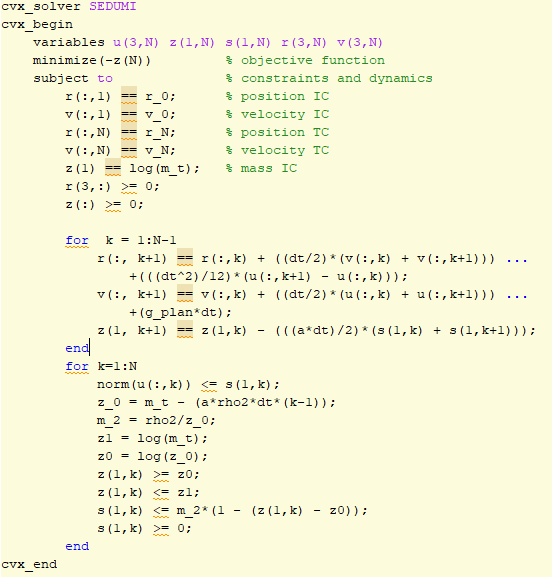
\includegraphics[scale= 0.6]{CVX.png}
  \caption{CVX script}
  \label{CVX}
\end{figure}
\clearpage


% NOW TO DO THE RESULTS PAGE!!!!!!
% 
% 

\begin{singlespace}
\section{RESULTS}
For many of the different stages of analysis, offline I generated an arbitrary trajectory (the helix) as it has many applications to drone missions, namely mapping objects. Additionally, this demonstrates the ability to conform to a changing trajectory, which is ultimately required for my convex optimal guidance. I will show functionality and accuracy at each of the key portions: LQR, LQG, the EKF, and the LQG with convex guidance all together.

\subsection{LQR Performance with Offline Trajectories}
LQR by itself worked quite well with following an offline trajectory. \ref{LQR} shows the commanded trajectory in orange and the flight path of the vehicle in blue. Additionally, the first point is marked with a green circle and the last point is a red circle.
\begin{figure}[!htpb]
\begin{subfigure}{.5\textwidth}
  \centering
	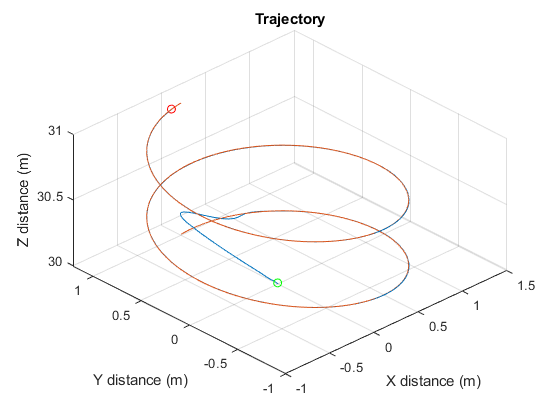
\includegraphics[scale= 0.5]{LQR.png}
	\caption{Convergence of just LQR in Offline Helix 1}
	\label{LQR}
\end{subfigure}%
\begin{subfigure}{.5\textwidth}
  	\centering
  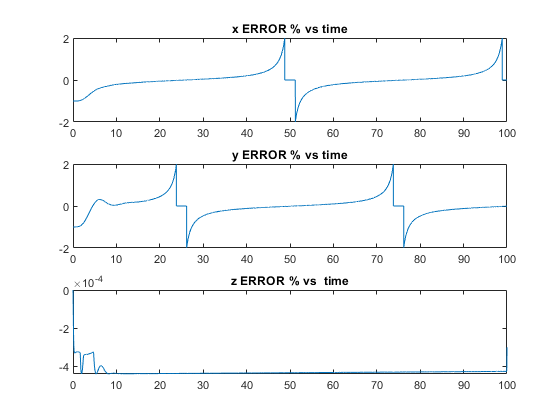
\includegraphics[scale= 0.65]{LQRerror.png}
  \caption{State error over time in the LQR case}
  \label{LQR_error}
\end{subfigure}%
\end{figure}



In figure \ref{LQR_error} we see the error of the system as it is being driven towards the commanded trajectory. In the $x$ and $y$ dimension it is always between positive and negative 2\%. In the $z$ dimension, the error converges to a steady state -0.0004\%. Also notice the singularities in error. This is because the actual state is being driven to zero, and there is not a way to calculate what percent of 0 we are. Ignore this for now, it is just a consequence of the trajectory. The error in figs \ref{LQR_error}, \ref{LQGhelix_err1}, and \ref{LQGhelix_err2} are calculated via $\frac{actual-commanded}{commanded}$.

\subsection{LQG Performance with Offline Trajectories}
In figures \ref{LQGhelix} and \ref{LQGhelix_2} we see the performance of the LQR and EKF together in following two different helix trajectories. If you look closely you will see that the $z$ dimension does not quite catch up and therefore has steady state error. The error plots for both of these trajectories are figures \ref{LQGhelix_err1} and \ref{LQGhelix_err2}. The first error plot shows similar bounded error below 2\% in x and y. The $z$ error is consistently quite low, below -0.0004\%. In \ref{LQGhelix_err2} we see much more error on the $z$ axis as the controller converges towards the trajectory. This is because it overshoots much more than the first helix. Additionally, we see that $z$ in both situations has a steady state error.

\begin{figure}[!htpb]
\begin{subfigure}{.4\textwidth}
  \centering
  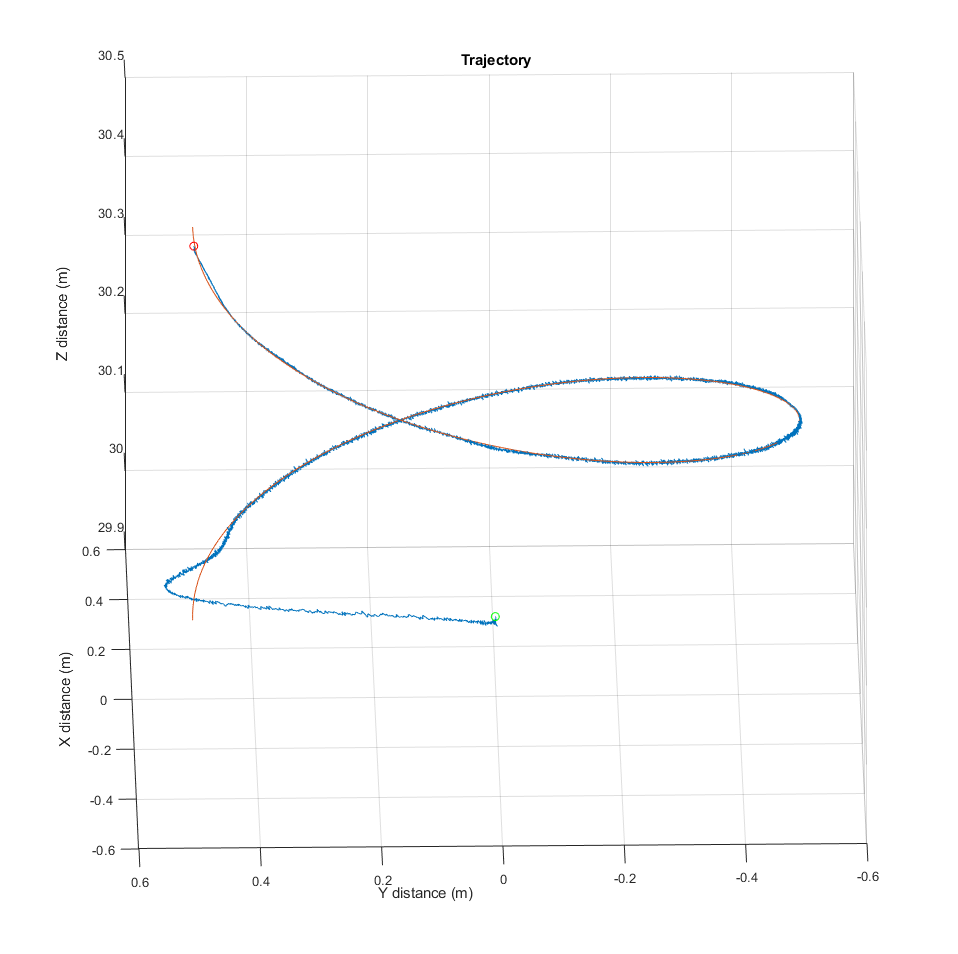
\includegraphics[scale= 0.3]{LQGhelix_1.png}
  \caption{First Helix trajectory under LQG control}
  \label{LQGhelix}
\end{subfigure}%
\begin{subfigure}{.4\textwidth}
  \centering
  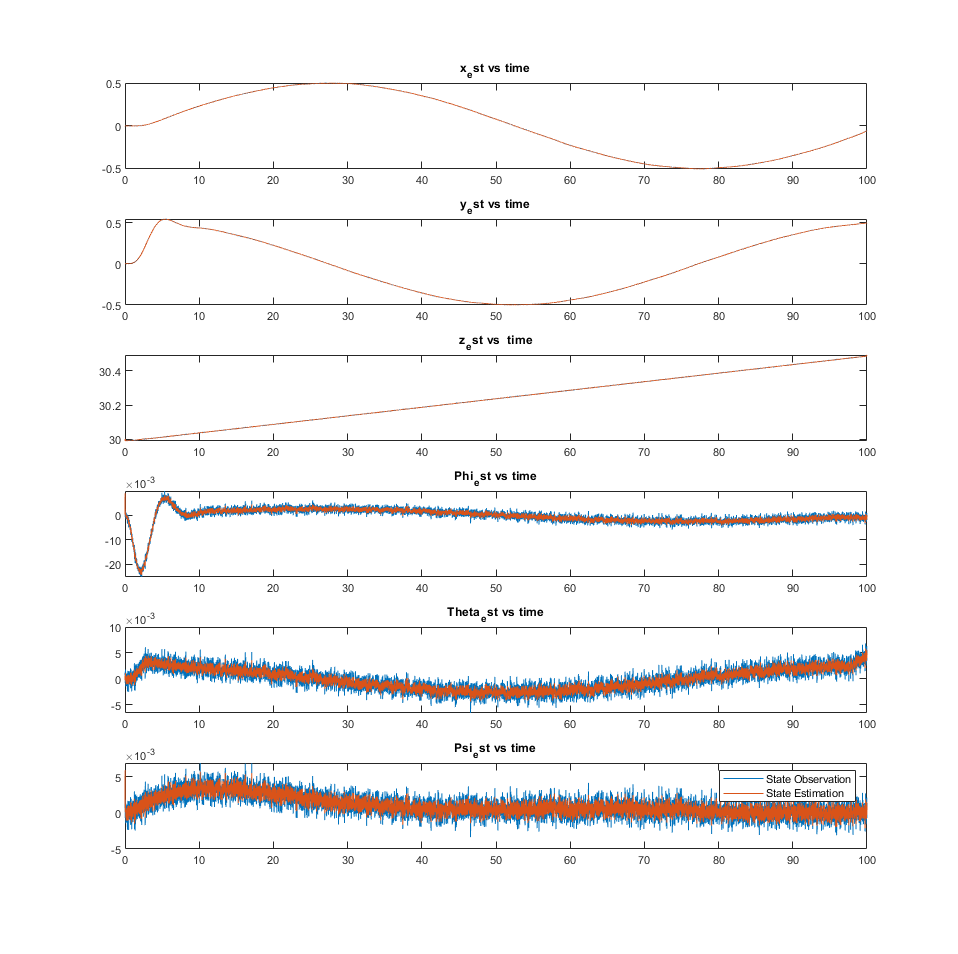
\includegraphics[scale= 0.4]{LQGhelix_1_state.png}
  \caption{States during first helix trajectory}
  \label{LQGhelix_1_state}
\end{subfigure}%
\end{figure}

\begin{figure}[!htpb]
\begin{subfigure}{.5\textwidth}
  \centering
  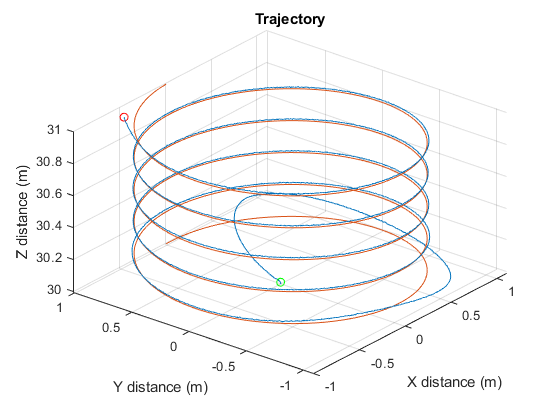
\includegraphics[scale= 0.65]{LQGhelix_2.png}
  \caption{Second Helix trajectory under LQG control}
  \label{LQGhelix_2}
\end{subfigure}%
\begin{subfigure}{.5\textwidth}
  \centering
  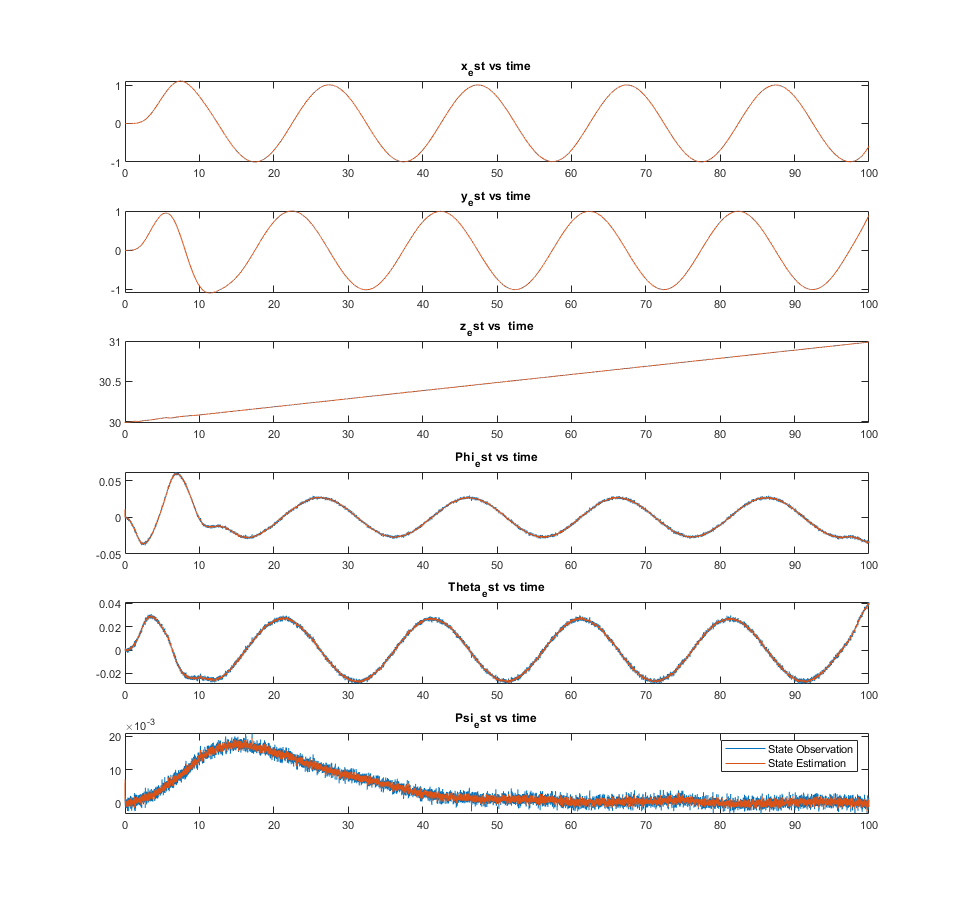
\includegraphics[scale= 0.4]{LQGhelix_2_state.png}
  \caption{States during second helix trajectory}
  \label{LQGhelix_2_state}
\end{subfigure}%
\end{figure}

\begin{figure}[!htpb]
\begin{subfigure}{.5\textwidth}
  \centering
  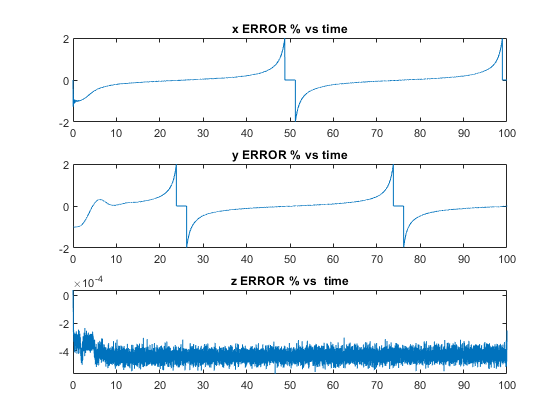
\includegraphics[scale= 0.6]{LQGhelix_1_err.png}
  \caption{Error in the first trajectory over time}
  \label{LQGhelix_err1}
\end{subfigure}%
\begin{subfigure}{.5\textwidth}
  \centering
  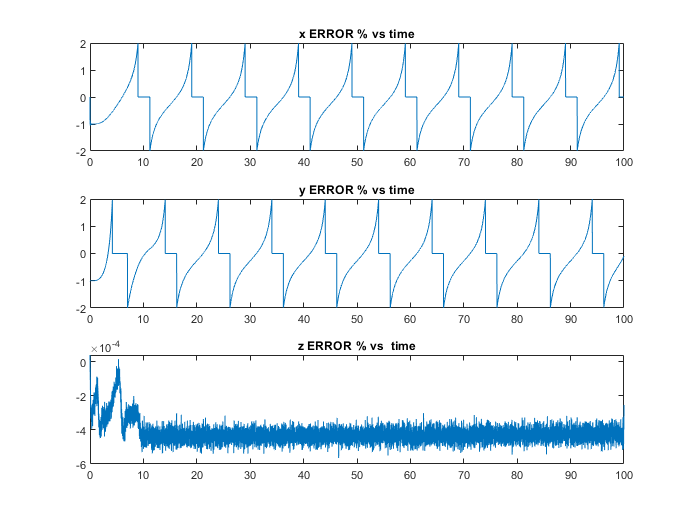
\includegraphics[scale= 0.5]{LQGhelix_2_err.png}
  \caption{Error in the second trajectory over time}
  \label{LQGhelix_err2}
\end{subfigure}%
\end{figure}


\subsection{EKF Convergence}
Figure \ref{LQGhelix_1_state} and \ref{LQGhelix_2_state} show the state variations as the vehicle travels through the helix. The state has been filtered through the EKF. The orange line is the filtered data while the blue line is the state as observed. I felt that the EKF worked quite well at converging close to the real state of the vehicle. In figure \ref{EKFerr2} we see the error in position throughout the 100 seconds. The $x$ and $y$ dimension error is between $+/-$1\%. The $z$ dimension error is centered around 0\% and is very small. This error is calculated in the same was as we calculated the trajectory error in previous sections.

\begin{figure}[!htpb]
\centering
  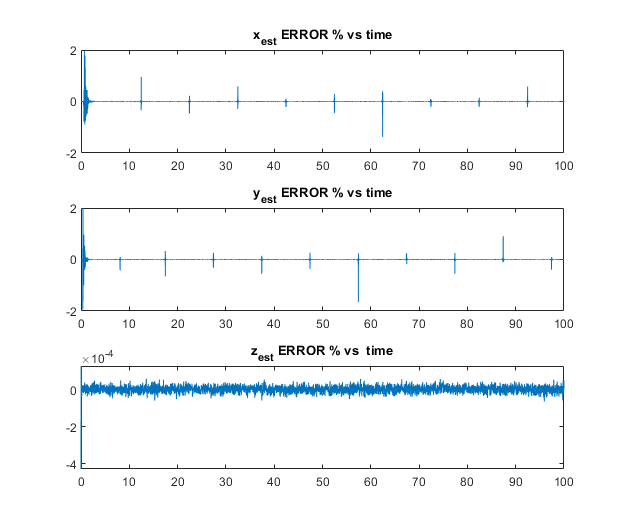
\includegraphics[scale= 0.6]{EKFerr2.png}
  \caption{EKF error through second trajectory}
  \label{EKFerr2}
\end{figure}

\subsection{LQG with Convex Optimal Trajectories}
In figure \ref{CVXpath}, we see an optimal trajectory with thrust vector quivers showing a trajectory from one point to another in the same plane with zero velocity initial condition. In figure \ref{LQGcvx}, we see the quadrotor attempting to follow the trajectory with the LQG controller. I was still having some trouble with CVX by the time this report was due unfortunately.

\begin{figure}[!htpb]
\begin{subfigure}{.5\textwidth}
  \centering
  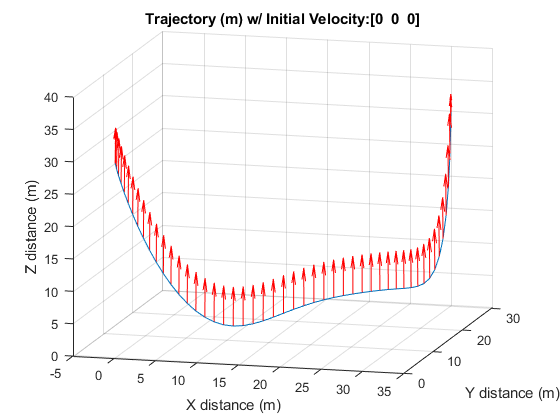
\includegraphics[scale= 0.6]{cvx_path.png}
  \caption{CVX generated path with red quivers denoting the thrust vector}
  \label{CVXpath}
\end{subfigure}%
\begin{subfigure}{.5\textwidth}
  \centering
  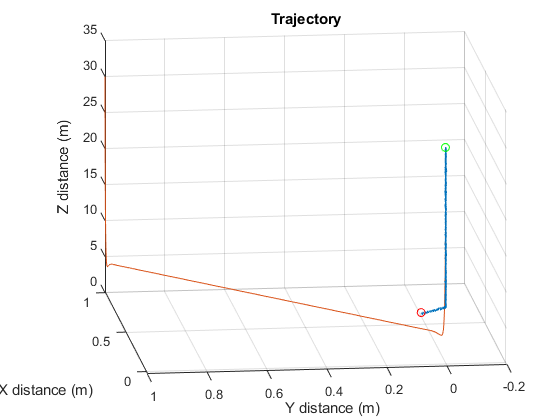
\includegraphics[scale= 0.5]{uhoh.png}
  \caption{LQG with CVX}
  \label{LQGcvx}
\end{subfigure}%
\end{figure}
\end{singlespace}





\section{Conclusions}
Overall, I think that my LQG solution worked well and I learned quite a bit from the process. Although my CVX algorithm generated optimal paths, I had trouble getting them to the time resolution required by the model. This should have involved some interpolation but I ran out of time. I think that I could have added PI compensation to improve the steady state error. Additionally, I could have tinkered more with the EKF variables such that it converged much more nicely in the $x$ and $y$ dimensions. I also could have decreased the frequency of the additive noise to a more reasonable quantity. If I had more time, I would have worked more on the convex problem to make it resemble an electrical power optimization more than a minimum-fuel problem. 


\clearpage
\end{doublespace}
\bibliography{sample}
\end{document}
